\section{Programming with Data-Trace Types}
\label{subsec:dtt-2}

In this section we give an illustration of type-consistent programming
using data-trace types.
We will also describe how type-consistent programming can be done for
synchronization schemas in the next section.
% Similarly, we can describe a programming framework using synchronization schemas, and this is done in~\citeMain{pods21}, but we are not concerned with
% the particular abstraction here, just the fact that type consistent programming
% constructs can be given.
The semantics for a stream processing program consists of:
\begin{enumerate}
\item
the type $X$ of input data traces,
\item
the type $Y$ of output data traces, and
\item
a monotone mapping $\beta: X \to Y$ that specifies the cumulative output after having consumed a prefix of the input stream.
\end{enumerate}
The monotonicity requirement captures the idea that output items cannot be retracted after they have been omitted. Since $\beta$ takes an entire input history (data trace) as input, it can model stateful systems, where the output that is emitted at every step depends potentially on the entire input history.

We have already discussed how (monotone) functions from $A^*$ to $B^*$ model sequential stream processors. We will now introduce the formal notion of \emph{consistency}, which captures the intuition that a sequential implementation does not depend on the relative order of any two elements unless the stream type considers them to be relatively ordered.

\begin{definition}[Consistency]
Let $X = (A,D)$ and $Y = (B,E)$ be data-trace types. We say that a data-string transduction $f: A^* \to B^*$
is \emph{$(X,Y)$-consistent} if $u \eq_D v$ implies that $\bar{f}(u) \eq_{E} \bar{f}(v)$ for all $u, v \in A^*$.

Let $f \in A^* \to B^*$ be a $(X,Y)$-consistent data-string transduction. The function $\beta: X \to Y$, defined by
$\beta([u]) = [\bar f(u)]$ for all $u \in A^*$, is called the \emph{$(X,Y)$-denotation} of $f$.
\end{definition}

\begin{definition}[Data-Trace Transductions]
Let $X = (A,D)$ and $Y = (B,E)$ be data-trace types. A \textbf{\em data-trace transduction} with input type $X$ and output type $Y$ is a function $\beta: X \to Y$ that is monotone w.r.t.\ the prefix order on data traces: $\trc u \leq \trc v$ implies that $\beta(\trc u) \leq \beta(\trc v)$ for all traces $\trc u, \trc v \in X$.
\end{definition}

It is shown in \citeMain{festschrift18} that the set of data-trace transductions from $X$ to $Y$ is equal to the set of $(X,Y)$-denotations of all $(X,Y)$-consistent data-string transductions.

We define two kinds of \textbf{\em data-trace types} for streams of key-value pairs: \emph{unordered} types of the form $\Unord(K,V)$, and \emph{ordered} types of the form $\Ord(K,V)$. For a set of keys $K$ and a set of values $V$, let $\Unord(K, V)$ denote the type with alphabet $K \cup \{\tg\#\}$, values $V$ for every key, values $\Nat$ for the $\tg\#$ tag (i.e., marker timestamps), and dependence relation $\{ (\tg\#, \tg\#) \} \cup \{ (k,\tg\#), (\tg\#,k) \mid k \in K \}$. In other words, $\Unord(K, V)$ consists of data traces where the marker tags $\tg\#$ are linearly ordered and the elements between two such tags are of the form $(k,v)$, where $k \in K$ and $v \in V$, and are completely unordered. We define $\Ord(K, V)$ similarly, with the difference that the dependence relation also contains $\{ (k,k) \mid k \in K \}$. That is, in a data trace of $\Ord(K,V)$, elements with the same key are linearly ordered between $\tg\#$ markers, but there is no order across elements of different keys.

A \textbf{\em transduction DAG} is a tuple $(S,N,T,E,\to,\lambda)$ which represents a labelled directed acyclic graph, where: $S$ is the set of \emph{source vertices}, $T$ is the set of \emph{sink vertices}, $N$ is the set of \emph{processing vertices}, $E$ is the set of \emph{edges} (i.e., connections/channels), $\to$ is the \emph{edge relation}, and $\lambda$ is a \emph{labelling function}. The function $\lambda$ assigns: (1) a data-trace type to each edge, (2) a data-trace transduction to each processing vertex that respects the input/output types, and (3) names to the source/sink vertices. We require additionally that each source vertex has exactly one outgoing edge, and each sink vertex has exactly one incoming edge.

\begin{example}[Time-Series Interpolation]
\label{ex:IoT}
Consider a home IoT system where temperature sensors are installed at a residence. We wish to analyze the sensor time series to create real-time notifications for excessive energy loss through the windows. The sensor time series sometimes have missing data points, and therefore the application requires a pre-processing step to fill in any missing measurements using linear interpolation. We assume that the sensors first send their measurements to a hub, and then the hub propagates them to the stream processing system. The stream that arrives from the hub does not guarantee that the measurements are sent in linear order (e.g., with respect to a timestamp field). Instead, it produces synchronization markers every 10 seconds with the guarantee that all elements with timestamps $< 10 \cdot i$ have been emitted by the time the $i$-th marker is emitted. That is, the $i$-th marker can be thought of as a watermark with timestamp $10 \cdot i$. The input stream is a data trace of $\Unord(\Ut,\texttt{M})$, where $\texttt{M}$ is the type of measurements $(\mathit{id}, \mathit{value}, \mathit{ts})$ consisting of a sensor identifier $id$, a scalar value $value$, and a timestamp $ts$. This is a transduction DAG that describes the pre-processing computation:
\newline
\centerline{%
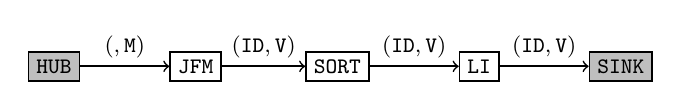
\begin{tikzpicture}[->, >=to, auto, node distance=1.8cm, semithick, transform shape]
%
\footnotesize
%
\node (A) [draw, fill=lightgray] {\texttt{HUB}};
\node (B) [draw, right of=A] {\texttt{JFM}};
\node (C) [draw, right of=B] {\texttt{SORT}};
\node (D) [draw, right of=C] {\texttt{LI}};
\node (E) [draw, fill=lightgray, right of=D] {\texttt{SINK}};
%
\path (A) edge node {$\Unord(\Ut,\texttt{M})$} (B);
\path (B) edge node {$\Unord(\texttt{ID},\texttt{V})$} (C);
\path (C) edge node {$\Ord(\texttt{ID},\texttt{V})$} (D);
\path (D) edge node {$\Ord(\texttt{ID},\texttt{V})$} (E);
%
\end{tikzpicture}
}% end of centerline
\newline
The vertex \texttt{HUB} represents the source of sensor measurements, and the vertex \texttt{SINK} represents the destination of the output stream. \texttt{ID} is the type of sensor identifiers, and \texttt{V} is the type of timestamped values $(\mathit{value}, \mathit{ts})$. The processing vertices are described below:
\begin{itemize}
\item
The stage Join-Filter-Map (\texttt{JFM}) joins the input stream with a table that indicates the location of each sensor, filters out all sensors except for those that are close to windows, and reorganizes the fields of the input tuple.
\item
Recall the guarantee for the synchronization markers, and notice that it implies the following property for the input traces: for any two input measurements that are separated by at least one marker, the one on the left has a strictly smaller timestamp than the one on the right. The sorting stage \texttt{SORT} sorts for each sensor the measurements that are contained between markers.
\item
The linear interpolation stage \texttt{LI} considers each sensor independently and fills in any missing data points.
\end{itemize}
We have described informally the data-trace transductions \texttt{JFM}, \texttt{SORT} and \texttt{LI}. The transduction DAG shown earlier denotes a data-trace transduction $\Unord(\Ut,\texttt{M}) \to \Ord(\texttt{ID},\texttt{V})$.
\end{example}

The computation performed by a processing node is given in a structured fashion, by completing function definitions of a specified \textbf{\em operator template}. We describe the three templates that are supported below, which encompass both ordered and unordered input streams. Each operator is defined by a sequential implementation. This means that each operator can be modeled as a data-string transduction. It can then be proved formally that these data-string transductions are consistent w.r.t.\ their input/output data-trace types. It follows that each operator that is programmed according to the template conventions has a denotation (semantics) as a data-trace transduction of the appropriate type.

\begin{itemize}
\item \texttt{OpStateless}:
The simplest template concerns \emph{stateless} computations, where only the current input event---not the input history---determines the output. The programmer fills in two function definitions: (1) \texttt{onItem} for processing key-value pairs, and (2) \text{onMarker} for processing synchronization markers. The functions have no output (the output type is \texttt{Ut}, i.e.\ the unit type) and their only side-effect is emitting output key-value pairs to the output channel by invoking $\texttt{emit(outputKey, outputValue)}$.

\item \texttt{OpKeyedOrdered}:
Assuming that the input is ordered per key, this template describes a stateful computation for each key independently that is order-dependent. The programmer fills in three function definitions: (1) \texttt{initialState} for obtaining the initial state, (2) \texttt{onItem} for processing a key-value pair and updating the state, and (3) \texttt{onMarker} for processing a synchronization marker and updating the state. The functions have output $S$, which is the type of the data structure for representing the state. As for stateless computations, the functions allow the side-effect of emitting output key-value pairs to the output channel. This template requires a crucial \emph{restriction} for maintaining the order for the output: every occurrence of \texttt{emit} must preserve the input key. If this restriction is violated, e.g.\ by projecting out the key, then the output cannot be viewed as being ordered.

\item \texttt{OpKeyedUnordered}:
Assuming that the input is unordered, this template describes a stateful computation for each key independently. Recall that the synchronization markers are ordered, but the key-value pairs between markers are \emph{unordered}. To guarantee that the computation does not depend on some arbitrary linear ordering of the key-value pairs, their processing does not update the state. Instead, the key-value pairs between two consecutive markers are aggregated using the operation of a \emph{commutative monoid} $A$: the programmer specifies an identity element $\texttt{id()}$, and a binary operation $\texttt{combine()}$ that must be \emph{associative} and \emph{commutative}. Whenever the next synchronization marker is seen, \texttt{updateState} is used to incorporate the aggregate (of type $A$) into the state (of type $S$) and then \texttt{onMarker} is invoked to (potentially) emit output. The behavior \texttt{onItem} may depend on the last snapshot of the state, i.e.\ the one that was formed at the last marker. The functions \texttt{onItem} and \texttt{onMarker} are allowed to emit output data items (but not markers), but the rest of the functions must be pure (i.e., no side-effects).
\end{itemize}

\begin{theorem}
\normalfont
Every streaming computation defined using the operator templates above is consistent w.r.t.\ its input/output type.
\end{theorem}

\section{Programming with Synchronization Schemas}
